%% TODO noch schreiben
\chapter{Ausblick}
\label{ch:ausblick}
Wie kann es weiter gehen? Was kann man noch machen? Was kann man ändern/hinzufügen?

\colorbox{yellow}{Hier fehlt was}

%% TODO noch schreiben
\section{Kompletter Workflow}
Daten in Maschine generrieren, IoT hochladen, in Maschine Learning über Connections einbauen und immer wieder
trainieren.

Allerdings sind automatisierte Tests nicht immer und für jede Anwendung geeignet. Michael Lüttel von der Deutschen 
Flugsicherung sagte auf der iqnite-Konferenz in Düsseldorf \enquote{Automatisierung macht nur dann Sinn, wenn sie mehr 
Aufwände einspart als sie selbst erzeugt.}\footnote{https://www.qz-online.de/news/uebersicht/nachrichten/vor-und-nachteile-von-automatisierten-software-tests-890130.html}

\colorbox{yellow}{Hier fehlt was}

\begin{figure}[h]
    \centering
    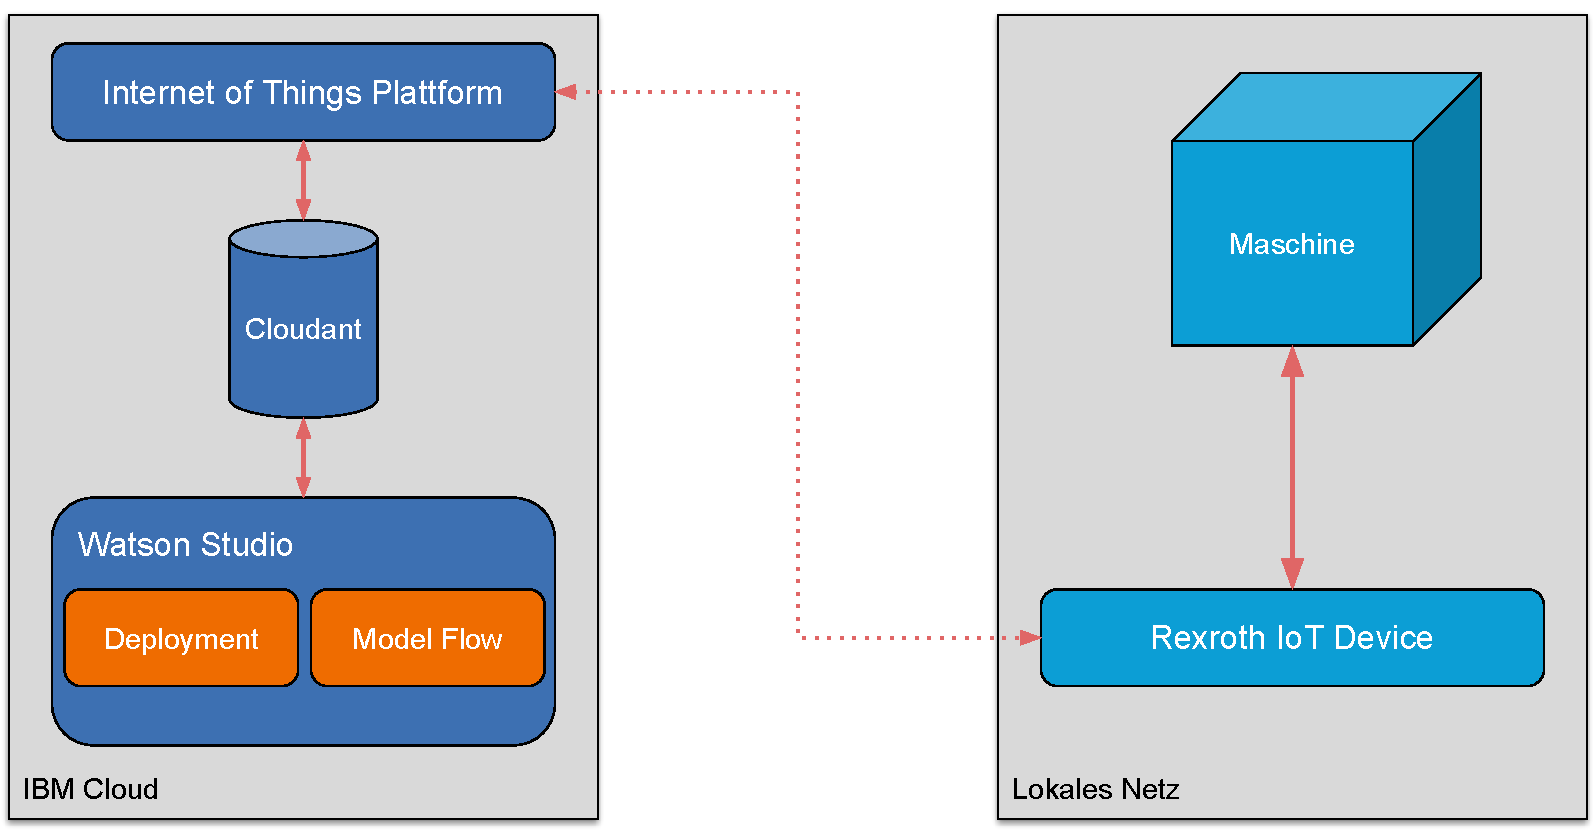
\includegraphics[width=\textwidth]{images/kapitel_6/architektur_uebersicht.pdf}
    \caption{Übersicht der Zielarchitektur}
    \label{fig:ausblick_uebersicht}
\end{figure}

%% TODO noch schreiben
\section{Function as a Service}
Wie könnte man Functions/Lambda einbauen. FaaS

\colorbox{yellow}{Hier fehlt was}

%% TODO noch schreiben
\section{Machine Learning für Smartphones}
Wie könnte man das Feature nutzen und was würde das bringen

\colorbox{yellow}{Hier fehlt was}

%% TODO noch schreiben
\section{Offline Modus}
Ein Offline-Mode für die Website mit TensorFlow.js.

\colorbox{yellow}{Hier fehlt was}

%% TODO noch schreiben
\section{AI OpenScale}
\label{ai_openscale}
Hiermit kann man veranschaulichen, warum und wie die AI auf das Ergebnis gekommen ist. Das kann man mit dem Deployment
und mit dem TensorFlow.js Ding machen. Dafür braucht man eine Datenbank.

\colorbox{yellow}{Hier fehlt was}

%% TODO nosch schreiben
\section{Docker-Container}
Das Frontend oder auch das Backend in einen Docker-Container packen. Zusammen mit der Schnittstelle.

\colorbox{yellow}{Hier fehlt was}

%% TODO nosch schreiben
\section{Skalierbarkeit}
Wie könnte man die Anwendung skalieren?

\colorbox{yellow}{Hier fehlt was}

%% TODO noch schreiben
\section{Audit mit Blockchain}
Für die Waage muss Audit gemacht werden. Könnte man Blockchian da nicht noch einbauen?

\colorbox{yellow}{Hier fehlt was}

%% TODO noch schreiben
\section{Nutzen von IoT}
Nutzen von IoT

\colorbox{yellow}{Hier fehlt was}

\begin{figure}[h]
    \centering
    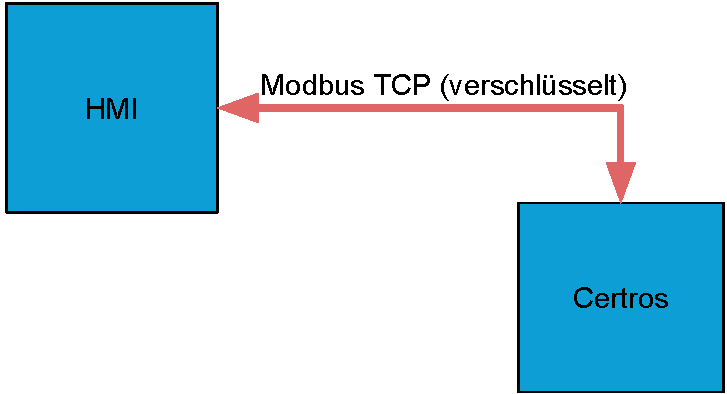
\includegraphics[width=\textwidth]{images/kapitel_6/iot_waage.pdf}
    \caption{Übersicht der Zielarchitektur}
    \label{fig:ausblick_iot}
\end{figure}

%% TODO noch schreiben
\subsection{Daten einlesen}
Wie könnten die Daten, welche durch das Netzwerk herausgefunden werden, auch automatisch in die Machine eingegeben werden?

\colorbox{yellow}{Hier fehlt was}

%% TODO noch schreiben
\subsection{Daten auslesen}
Wie könnte man Daten der Maschine auslesen, damit man sie nutzen kann um das Neuronale Netz weiter zu verbessern?

\colorbox{yellow}{Hier fehlt was}